\documentclass[journal]{IEEEtran}
\usepackage[utf8]{inputenc}
\usepackage{blindtext}
\let\labelindent\relax
\usepackage[inline]{enumitem}
%\usepackage{enumerate}
\usepackage{graphicx}
\usepackage[shortcuts,acronym]{glossaries}
\usepackage{subcaption}
\usepackage[bookmarksopen, bookmarksdepth=2, breaklinks=true]{hyperref}

% *** GRAPHICS RELATED PACKAGES ***
\ifCLASSINFOpdf
\else
\fi
\makeglossaries
\newacronym{HMI}{HMI}{Human Machine Interaction}
\hyphenation{op-tical net-works semi-conduc-tor}


\begin{document}	
	\title{Workshop: Verbesserung der Mensch-Maschinen-Interaktion durch Emotion Tracking}
	
	\author{\begin{center}
			\begin{tabular}{c c} 
				Marius Becherer & Michael Zipperle \\ 
				\textit{259158} & \textit{259564} \\
				Marius.Becherer@hs-furtwangen.de & Michael.Zipperle@hs-furtwangen.de \\
			\end{tabular}
	\end{center}}%
	
	%\author{Christian Laustsen, \textit{20176018},
	%        Anders Rikvold, \textit{20176009},
	%        and Michael Zipperle, \textit{20176059}}% <-this % stops a space
	%\thanks{M. Shell is with the Department
	%of Electrical and Computer Engineering, Georgia Institute of Technology, Atlanta,
	%GA, 30332 USA e-mail: (see http://www.michaelshell.org/contact.html).}% <-this % stops a space
	%\thanks{J. Doe and J. Doe are with Anonymous University.}% <-this % stops a space
	%\thanks{Manuscript received April 19, 2005; revised January 11, 2007.}}
	
	% The paper headers
	\markboth{Hochschule Furtwangen - Ergonomie, June 2018}%
	{Hochschule Furtwangen - Ergonomie, June 2018}
	
	% make the title area
	\maketitle
	
	
	\begin{abstract}
		%\boldmath
		Bei den meisten Interaktionen zwischen Mensch und Maschine werden die Emotionen des Benutzers nicht in Betracht gezogen. Diese spielen jedoch eine wichtige Rolle, denn diese Beschreiben wie der Nutzer sich fühlt. Durch das Emotion Tracking kann die Information an die Emotionen eines Nutzers angepasst werden. Dies soll dazuführen, dass der Nutzer während der Interaktion mit der Maschine positive Emotionen aufweist. Somit kann durch Emotion Tracking eine Verbesserung der Mensch-Maschinen-Interaktion herbeigeführt werden. Dieser Artikel erläutert die theoretischen Grundlagen um die Emotionen eines Nutzers zu erkennen und darauf zu reagieren. Des Weiteren werden methodische Mittel beschrieben, wie diese Grundlagen einer Gruppe von Personen im Rahmen eines Workshops vermittelt werden und wie die Ergebnisse eines durchgeführten Workshops aussehen.
	\end{abstract}
	
	% Note that keywords are not normally used for peerreview papers.
	%\begin{IEEEkeywords}
	%IEEEtran, journal, \LaTeX, paper, template.
	%\end{IEEEkeywords}
	
	% For peerreview papers, this IEEEtran command inserts a page break and
	% creates the second title. It will be ignored for other modes.
	\IEEEpeerreviewmaketitle
	
	
	% *** START OF SECTIONS ***--------------------------------------------
	
	\section{Einführung}
Im heutigen Zeitalter muss nicht mehr allzu viel von Hand erledigt werden, denn für viele Anwendungen stehen Maschinen und sonstige Hilfsmittel bereit. Wir Menschen benutzen diese Geräte gerne, um uns den Alltag zu erleichtern. Bei der Kommunikation zwischen Menschen können Missverständnisse auftreten. In den meisten Fällen können diese anhand der Gestik und Mimik des Kommunikationspartners festgestellt werden und es kann entsprechend reagiert werden. Kommunizieren wir mit einer herkömmlichen Maschine, wie einem Computer, steht für die Eingabe meist nur eine Maus und Tastatur zur Verfügung. Dies bedeutet der Computer hat nicht die Möglichkeit, Missverständisse bei uns Menschen anhand unserer Gestik und Mimik, zu verstehen. Diese Missverständnisse führen oft zu Frust bei Menschen. In den Computerwissenschaften hat sich ein eigener Fachbereich gebildet, welcher sich mit der \ac{HMI} beschäftigt. Teilgebiete dieses Bereichs erforschen Methoden zum Feststellen des emotionalen Zustandes eines Menschen. Während seiner Interaktion mit einer Maschine, wodurch solche Missverständnisse erkannt und beseitigt werden können.

Dieser Artikel wurde im Rahmen des Faches Ergonomie im Studiengang Mobile Systeme an der Fachhochschule Furtwangen erstellt. Die Aufgabe war es einen 75-minütigen Workshop mit einer Dokumentation zu erstellen. Das Thema durfte frei im Bereich Ergonomie ausgewählt werden. Bei der Recherche nach einem geeigneten Thema, sind wir im Bereich Emotion Tracking und Affective Computing fündig geworden. Die Vision eine Kommunikation von Mensch zu Maschine an die Kommunikation von Mensch zu Mensch anzugleichen, überzeugte uns von dem Themengebiet, sodass wir den Artikel "A Suggestion to Improve User-Friendliness Based on Monitoring Computer User’s Emotions" ausgewählt haben \cite{EmotionTrackingGSR}. Der Inhalt des Artikels gliedert sich in grundlegenden Überlegungen zu Affective Computing und stellt eine Kombination von Emotion-Tracking-Methoden vor.

In den nachfolgenden Kapitel wird der Workshop genauer erläutert. Zunächst steht die Planung im Fokus. Hierbei wird die Recherche und deren Ergebnisse beschrieben, woraus die Agenda des Workshops entstand. Danach werden didaktische Methoden erarbeitet, um den Teilnehmern einen möglichst interessanten Workshop zu bieten und diese für das Thema zu motivieren. Das Kapitel Durchführung beschreibt den Workshopablauf, bei dem die theoretischen Inhalte und die Ergebnisse der Aufgaben dargestellt werden. In der anschließenden Evaluation wird ein Rückblick auf die Vorbereitung und Durchführung des Workshops gegeben. Dabei wird die Vorbereitung, der Inhalt und die didaktischen Methoden kritisch beurteilt.

	\section{Planung}


\subsection{Related Research / Recherche }

Nach der Bearbeitung des Artikels, konnte eine grobe Übersicht über das Thema gewonnen werden. Es stellt sich allerdings heraus, dass der Artikel kein Inhalt für einen 75 minütigen Workshop bot. Somit musst die Recherche erweitert werden, um ein höheres Abstraktionsniveau zu gewinnen. Zunächst untersuchten wir die zitierten Referenzen nach der Schneeballmethode. Hiermit konnte der Begriff Affective Computing\cite{Picard} nochmals verinnerlicht werden. Die genau Begriffsdefinition und die weiteren genannten Meilensteine, um das Ziel Affective Computing zu erreichen, sind sehr wichtig für das Verständnis der impliziten und expliziten Kanäle\cite{KimNS}. Für die verschiedene Methoden des Emotion Tracking sind ebenfalls Quellen angegeben\cite{cowie}\cite{zeng}\cite{lee}. Allerdings wurde die Recherche hier erweitert, sodass noch weitere Methoden, wie \cite{AutoEmotion} \cite{Carlos}. Im Bereich der Anwendungsfälle wird Affective Computing teilweise in der medizinischen Informatik\cite{medicine} und Sprachassisten\cite{sprachassi} angewendet. Eine beispielhafte Website, welche das Benutzerverhalten transparent überwacht und den Inhalt passenden dafür erzeugt, haben wir nicht gefunden. Es gibt jedoch einige Unterstützungen und Tools, wie Affectiva Emotion SDK\cite{affectiva} oder Microsoft Azure Cognitive Services\cite{MicrosoftAzure}, welche Affective Computing in einer Anwendung umsetzen soll.


\subsection{Agendaentwurf und Zeitplung}
Aufgrund dieser Recherche konnten wir ein Überblick über das Thema Affective Computing schaffen. Wir überlegten uns die Kernpunkte unseres Workshops und erstellten folgende fünf Fragen, welche die Teilnehmer nach dem Workshop beantworten können sollten:

\begin{itemize}
	\item Was sind Emotionen?
	\item Was ist Affective Computing?
	\item Welche Methoden gib es?
	\item Wie können diese Methoden in Anwendungen integriert werden?
	\item Welche Anwendungen setzen dies bereits um? 
\end{itemize}


Mit diesem Fragen wollten wir eine geeignete Agenda erstellen, welche vom Allgemeinen in die konkrete Methodik und Anwendung übergeht. Die Agenda bestand aus folgender Struktur, bei der die einzelnen Punkte mit einer ungefähren Zeit abgeschätzt wurde:

\begin{center}
	
\begin{tabular}{r l  l}
	1.&Motivation	&(15 min) \\
	2.&Ziel		&	(5 min) \\
	3.&Methoden	&	(30 min) \\
	4.&Umsetzung	&	(20 min) \\ 
	5.&Fazit		&	(10 min) \\
	6.&Diskussion	&(5 min) \\
\end{tabular}

\end{center}

Diese Agenda diente als Grundlage für die erste Besprechung. Bei einzelnen Punkten waren Änderungen notwendig, aber an dem Grundgerüst des Workshops gab es wenig zu bemängeln. Bevor wir nun den Workshop erstellten, haben wir uns nochmals in die Punkte der Agenda vertieft. 


\subsection{Methodik}  

Als Vorgabe für das didaktische Konzept wurde bereits der Workshop festgelegt, dessen Gestaltung war jedoch frei wählbar. Es stellte sich die Herausforderung entsprechende Methoden einzusetzen, welche sich positiv auf das Lernverhalten und die Motivation auswirken. Der Workshop sollte sich aus einem Vortrag zusammensetzen, welcher mit Gruppenaufgaben ergänzt wurde. Dabei soll der Vortrag Themen zusammenfassen und eine fundierte Basis liefern. In den Aufgaben soll dann das Wissen erweitert und ergänzt werden. Eingangs soll eine  Aufgabe in Einzelarbeit als Versuch durchgeführt werden, sodass die Teilnehmen für das Thema motiviert sind. Nach weiteren einführenden Informationen finden zwei Gruppenarbeiten statt, welche von den Workshopleitern betreut wird. Die Ergebnisse werden moderiert, sodass die Teilnehmer im Fokus stehen und eine erhöhte Aufmerksamkeit auf die Ergebnisse gegeben sein soll. Abschließend soll noch eine kurze Diskussion stattfinden, wobei die Teilnehmer ihr gesammeltes Wissen aus dem Workshop für die Diskussion transferieren können. Als Medien werden Beamer und Flipchart verwendet. Der Beamer soll die einzelnen Vortragsabschnitte unterstützen und die gesammelten Ergebnisse live präsentieren. Die Flipcharts können von der Gruppen zur Ergebnispräsentation verwendet werden. 




	\section{Durchführung}

\subsection{Motivation}


\subsubsection{Einleitung}

Die Workshopteilnehmer sollten zu Beginn für das Thema Affective Computing motiviert werden. Dafür gibt es einen kurze Beschreibung der Emotionen mit den Charakteristiken, wie zum Beispiel, dass Emotionen sehr schnell auftreten, aber dafür ebenfalls sehr ungenau sind. Die Intensität ist ebenfalls ein Merkmale der Emotionen. Eine hohe Intensität ist kurzzeitig und stark im Gegensatz zu einem niedrigen Intensiätsempfinden der Emotionen. Eine geringe Intensität ist dauert länger an und wird auch als Stimmung bezeichnet. 

\subsubsection{Workshop Aufgabe}\label{Workshop Aufgabe}



Ziel der Aufgabe ist es den verschiedenen Benutzerempfindlichkeiten aufzuzeigen. Die Aufgabe soll in zwei Gruppen erfolgen, bei der die Gruppen jeweils verschiedene Websiten angezeigt bekommen haben. Auf der Website sollten diese nach Informationen suchen, um den veröffentlichten Fragebogen auszufüllen. Anschlißend sollten die Emotionen eingetragen werden. Während Gruppe 1 ihre Informationen in Wikipedia recherchierte, durfte Gruppe 2 eine Website besuchen, welche den Inhalt grafisch ergänzt. Dabei zeigte sich folgende Auswertungen der Emotionen, welche in Abbildung 1 und Abbildung 2 dargestellt.

\begin{figure}[!h]
	\centering
	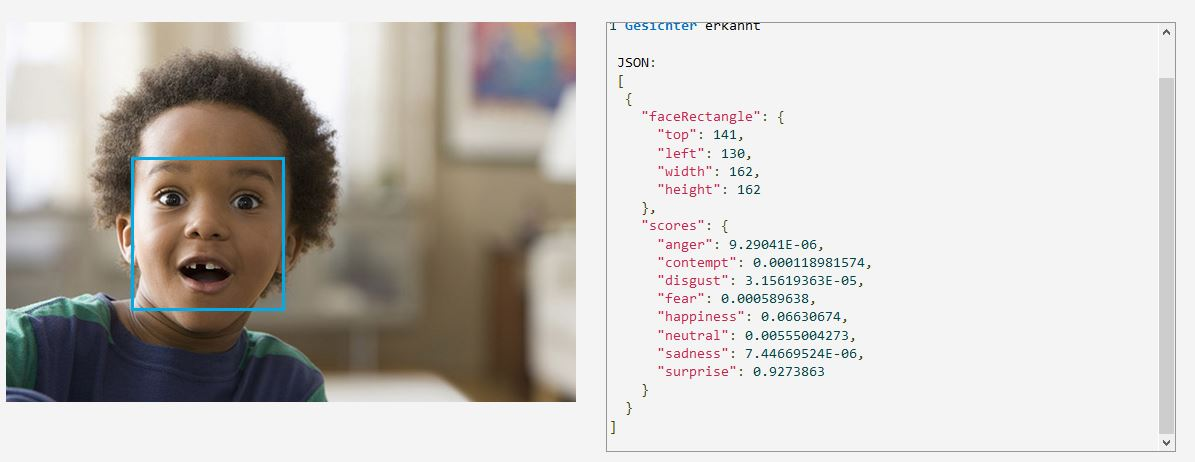
\includegraphics[width=0.9\linewidth]{Pictures/Microsoft_Gestenerkennung}
	\caption[Beispiel: Microsoft Azure Emotionserkennung]{Beispiel: Microsoft Azure Emotionserkennung \cite{MicrosoftAzure}}
	\label{fig:microsoftgestenerkennung}
\end{figure}

\subsection{Ziele}

Zu Beginn beschrieben wir den Ablauf einer \ac{HMI} Kommunikation. Dabei sahen die Teilnehmer, dass der Benutzer haptische und akustische Eingaben in das System tätigte und eine visuelle, akustische Ausgabe erhaltet. Diese Art der Kommunikation stellten wir als expliziten Kommunikationskanal vor. Dieser zeichnet sich durch die rationalen Informationen aus. Im Gegensatz hierzu stellt der implizite Kanal als Eingabe Emotionen zur Verfügung, worauf der Benutzer eine visuelle, akustische Ausgabe von seinem Kontext empfängt. Schließlich sollte als Eingabe eine haptische und akustische Eingabe der rationalen Informationen dienen, welche mit den Emotionen des Benutzers ergänzt wird, siehe Abbildung ~\ref{fig:communiationskanal}. Hiermit kann eine Anwendung auf die Empfindlichkeiten des Anwenders reagieren. 

\begin{figure}[!h]
	\centering
	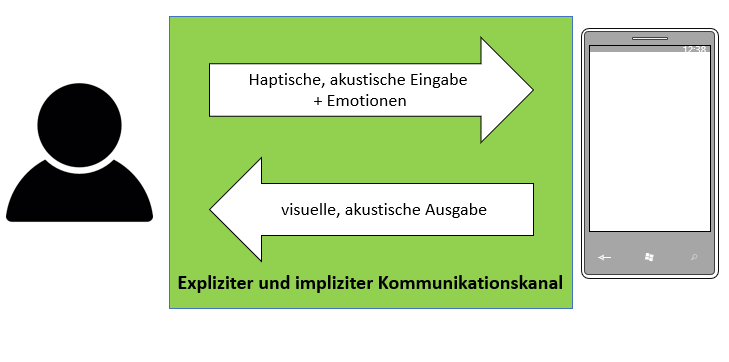
\includegraphics[width=0.9\linewidth]{Pictures/impliziter_expliziter_Kanal}
	\caption[Vereinigung des impliziten und expliziten Kommunikationskanal]{Vereinigung des impliziten und expliziten Kommunikationskanal}
	\label{fig:communiationskanal}
\end{figure}  

Anschließend wurde der Begriff "Affective Computing" eingeführt, der ein System beschreibt, welches Emotionen erkennen, interpretieren und verarbeiten kann. Dabei zeigten wir die von Picard beschrieben Punkte auf, um ein solches System umzusetzen:

\vspace{2mm}
\begin{enumerate}
	\item Frustration reduzieren
	\item Klassifizierung der Emotionen
	\item Infrastruktur für Affective Computing schaffen
	\item Emotionale Eigenschaften des Systems trainieren
\end{enumerate}
\vspace{2mm}

Zunächst ist es das übergeordnete Ziel die Frustration zu reduzieren. Hierfür können schon einfache Fehlermeldungen reichen, welche die Schuld auf sich nimmt. Für ein intelligenteres System braucht es allerdings noch verschiedene Sensoren, welche Benutzerdaten erfassen. Aus den gesammelten Daten soll nun versucht werden die Benutzeremotionen zu klassifizieren. Sobald das System die Emotionen klassifiziert hat, ist eine Antwort des Systems notwendig. Die Antwort soll natürlich in Zusammenhang mit dem gegebenen Kontext stehen, sodass der Benutzer zielgerichtet angesprochen werden kann.


\section{Umsetzung: Methoden}
\subsection{Methoden zum Emotion Tracking}
Es gibt verschiedene Methoden um die Emotion eines Nutzers während dessen Interaktion mit einer Maschine zu tracken. Im folgenden werden beispielhaft verschiedene Methoden erläutert:

\subsubsection{Hautwiderstand und Hauttemperatur}
Das Paper "A Suggestion to Improve User-Friendliness Based
on Monitoring Computer User’s Emotions" beschreibt, wie Emotionen eines Nutzers durch dessen Hauttemperatur und Hautwiderstand bestimmt werden können. Die Autoren nutzen dafür ein Temperatur- und Hautwiderstandssensor, die mit einem Arduino verbunden sind. Die Daten der Sensoren werden in einer SQLite Datenbank gespeichert und auf einer Android App ausgegeben. Die Autoren stellten fest, dass eine Änderung der Hauttemperatur bzw. des Hautwiderstands  auf eine Emotionsänderung des Nutzers zurückzuführen ist \cite{EmotionTrackingGSR}.

\subsubsection{Blick}
Die Autoren des Papers "Improving Human-Computer Interaction
by Gaze Tracking" untersuchten, wie das Tracken des Blickes des Nutzers zur Steuerung von Maschinen verwendet werden kann. Unter anderem konnte festgestellt werden, wo und wie lange der Nutzer ein Objekt auf der Maschine betrachtet. Dabei wurde festgestellt, dass durch dieses Verfahren auch die Emotionen eines Nutzers bestimmt werden können. Beispielsweise verändert sich die Pupillengröße bei einer Emotionsänderung des Nutzers. Dabei nutzen die Autoren die integrierte Webcam in einem Laptop, um den Blick und somit die Emotionen eines Nutzers zu Tracken. Somit wird keine zusätzliche Hardware benötigt, wenn das Endgerät des Nutzers bereits eine Kamera integriert hat \cite{EmotionTrackingGaze}.

\subsubsection{Gesichtsausdruck}
Cloud Service Anbieter wie Amazon, IBM und Microsoft bieten Cognitive Services an, darunter auch ein Service zur Emotionserkennung. Abbildung \ref{fig:microsoftgestenerkennung} zeigt eine Live Demo des Service von Microsoft, dabei wird die Emotion "Überraschung" mit einer Wahrscheinlichkeit von 0,93 erkannt. Bei der Live Demo kann ein Bild hochgeladen oder direkt wie Webcam aufgezeichnet werden. Der Service erkennt dann zuerst die Person bzw. Personen und bestimmt zu jeder Person, mit viel Prozent diese mit einer vorgegeben Emotionen übereinstimmt.

\begin{figure}[!h]
	\centering
	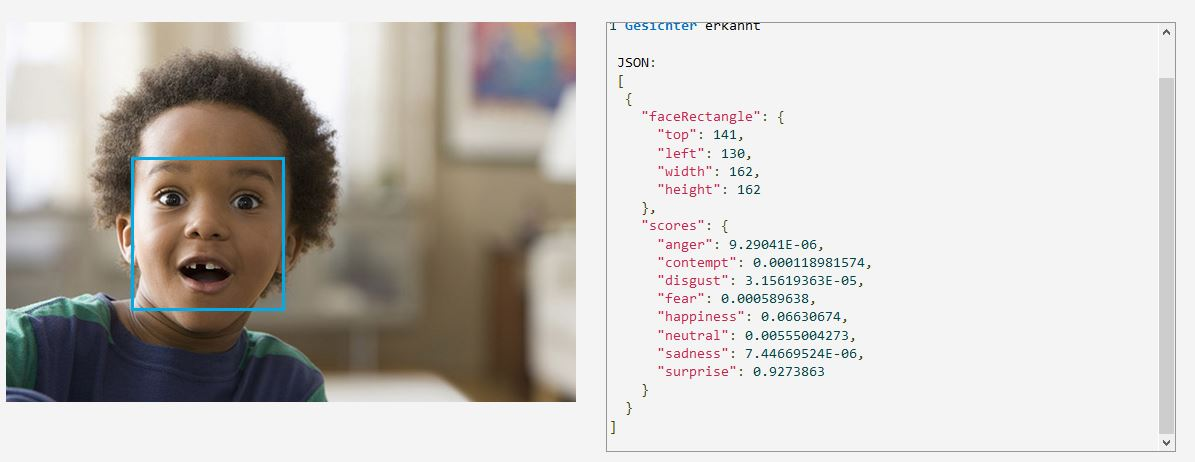
\includegraphics[width=0.9\linewidth]{Pictures/Microsoft_Gestenerkennung}
	\caption[Beispiel: Microsoft Azure Emotionserkennung]{Beispiel: Microsoft Azure Emotionserkennung \cite{MicrosoftAzure}}
	\label{fig:microsoftgestenerkennung}
\end{figure}

\subsubsection{Sprachinformationen}
Die Emotionen eines Menschen spiegeln sich in der Sprache dessen wieder. Ein typisches Beispiel hierfür ist, wenn eine Person einen Vortrag hält und dabei sehr verunsichert und aufgeregt ist, die Person spricht oft schnell und verspricht sich gegebenenfalls. Die Autoren des Papers "Speech emotion recognition approaches in human computer interactiong" untersuchten, wie genau können Emotionen eines Nutzers durch die Sprachinformationen bestimmt werden. Dabei extrahierten diese Muster aus mehreren Sprachsignal und bestimmten für dieses Muster die Emotionen des Sprechers. Diese Informationen wurden dann verwendet, um eine künstliche Intelligenz zu trainieren, um somit für ein beliebiges Sprachsignale die zugehörige Emotion vorherzusagen \cite{SpeechInformation}.

\subsection{title}
\section{Umsetzung: Andwendungsfälle}\label{Umsetzung_Anwendungsfaelle}
Im letzten Kapitel wurden Methoden aufgezeigt, um die Emotionen eines Nutzer während dessen Interaktion mit einer Maschine zu tracken. In diesem Kapitel gilt es herauszufinden, wie das Wissen über die Emotionen eines Nutzers genutzt werden kann, um die Interaktion zwischen Mensch und Maschine zu verbessern. Dazu sollen Anwendungsfälle aufgezeigt werden, bei denen die Nutzung von Emotion Tracking ein Vorteil aufbringt. Für dieses Kapitel ist keine theoretisches Wissen nötig und es kann somit direkt zu einer interaktiven Aufgabe mit den Teilnehmern des Workshops übergegangen werden.

\subsection{Workshop Aufgabe}
Insgesamt waren es drei Gruppen a vier Personen, jeder Gruppe wurde eine der folgenden Emotion Tracking Methode zugewiesen:

\begin{itemize}
	\item Gesichtsausdruck
	\item Sprachinformation
	\item Hauttemperatur
\end{itemize}
Die Gruppen wurden aufgefordert, folgende Aufgabe durchzuführen.
\begin{itemize}
	\item Gruppengröße: 4 Personen
	\item Bearbeitungszeit: 20 Minuten
	\item Arbeitsverfahren: Recherche & Entwicklung
	\item Beschreibung: Die folgenden Aufgaben sind in Bezug zu einer bestimmten Emotion Tracking Methode zu bearbeiten:
	\begin{enumerate}
		\item Recherchieren Sie nach bestehenden Anwendungsfällen, bei denen Emotion Tracking zur Verbesserung der HMI eingesetzt wird.
		\item Überlegen Sie sich Anwendungsfälle, bei denen Emotion Tracking zur Verbesserung der HMI eingesetzt werden könnte.
		\item Welche Vor- und Nachteile der Ihnen zugeteilten Methode kommen auf.
	\end{enumerate}
\end{itemize}

Nach Bearbeitung der Aufgabe, wurden jede Gruppe aufgefordert ihre Ergebnisse mit Hilfe des Plakats den anderen Workshop Teilnehmer zu präsentieren.

\subsection{Workshop Ergebnisse}\label{Umsetzung_Anwendungsfaelle_Ergebnisse}
	\section{Evaluation}
Der Workshop ist nach unserer Einschätzung bei den Teilnehmern gut angekommen. Die fünf Leitfragen, welche in Abschnitt II.B formuliert wurden, haben uns dabei geholfen einen Workshop zu erstellen, der nicht vom eigentlichen Thema abweicht. 
In der Feedback Runde wurde der Aufbau des Workshops positiv aufgenommen. Durch die Mischung aus kurzen Vorträgen und längeren Gruppenarbeit konnten wir die Teilnehmer für dieses Thema begeistern. Wir denken es war der richtig, ein Fundament zu schaffen, auf dem schließlich in Einzel- oder Gruppenarbeit aufgebaut werden konnte. 
Die ausgewählten didaktischen Methoden sind an den richtigen Stellen zum Einsatz gekommen. Bei der zweiten und dritten Aufgabe konnten die Teilnehmer zielgerichtet arbeiten und sind zu guten Ergebnissen gekommen. Es wurden sogar noch weitere Methoden entdeckt, welche wir in unserer Recherche nicht gefunden hatten.  Die erste Aufgabe, die als Einstieg für die Motivation gelten sollte, war mittelmäßig. Ziel war es zu zeigen, dass Benutzer verschieden sind. Durch die Einteilung in zwei Gruppen mit einem negativen und positiven Beispiel konnte ein Versuch durchgeführt werden, der zwar unser erwartetes Ergebnis bestätigte, aber vermutlich konnten eine Gruppe nicht allzu sehr motiviert werden, da unser Negativbeispiel auch nicht Spaß machen sollte. In Zukunft wäre eine Aufgabe, welche die komplette Gruppe motiviert, besser gewesen. 
Zusammengefasst kann gesagt werden, dass wir mit unserem Workshop sehr zufrieden waren. Wir haben festgestellt, dass die eigentliche Aufgabe in einer umfangreichen Recherche liegt, um das Thema richtig zu verstehen. Gelingt dies, lässt sich die Struktur und der Inhalt für den Workshop schnell erstellen.
  
	
	
	
	% *** END OF SECTIONS ***---------------------------------------------
	
	% needed in second column of first page if using \IEEEpubid
	%\IEEEpubidadjcol
	
	% An example of a floating figure using the graphicx package.
	% Note that \label must occur AFTER (or within) \caption.
	% For figures, \caption should occur after the \includegraphics.
	% Note that IEEEtran v1.7 and later has special internal code that
	% is designed to preserve the operation of \label within \caption
	% even when the captionsoff option is in effect. However, because
	% of issues like this, it may be the safest practice to put all your
	% \label just after \caption rather than within \caption{}.
	%
	% Reminder: the "draftcls" or "draftclsnofoot", not "draft", class
	% option should be used if it is desired that the figures are to be
	% displayed while in draft mode.
	%
	%\begin{figure}[!t]
	%\centering
	%\includegraphics[width=2.5in]{myfigure}
	% where an .eps filename suffix will be assumed under latex, 
	% and a .pdf suffix will be assumed for pdflatex; or what has been declared
	% via \DeclareGraphicsExtensions.
	%\caption{Simulation Results}
	%\label{fig_sim}
	%\end{figure}
	
	% Note that IEEE typically puts floats only at the top, even when this
	% results in a large percentage of a column being occupied by floats.
	
	
	% An example of a double column floating figure using two subfigures.
	% (The subfig.sty package must be loaded for this to work.)
	% The subfigure \label commands are set within each subfloat command, the
	% \label for the overall figure must come after \caption.
	% \hfil must be used as a separator to get equal spacing.
	% The subfigure.sty package works much the same way, except \subfigure is
	% used instead of \subfloat.
	%
	%\begin{figure*}[!t]
	%\centerline{\subfloat[Case I]\includegraphics[width=2.5in]{subfigcase1}%
	%\label{fig_first_case}}
	%\hfil
	%\subfloat[Case II]{\includegraphics[width=2.5in]{subfigcase2}%
	%\label{fig_second_case}}}
	%\caption{Simulation results}
	%\label{fig_sim}
	%\end{figure*}
	%
	% Note that often IEEE papers with subfigures do not employ subfigure
	% captions (using the optional argument to \subfloat), but instead will
	% reference/describe all of them (a), (b), etc., within the main caption.
	
	
	% An example of a floating table. Note that, for IEEE style tables, the 
	% \caption command should come BEFORE the table. Table text will default to
	% \footnotesize as IEEE normally uses this smaller font for tables.
	% The \label must come after \caption as always.
	%
	%\begin{table}[!t]
	%% increase table row spacing, adjust to taste
	%\renewcommand{\arraystretch}{1.3}
	% if using array.sty, it might be a good idea to tweak the value of
	% \extrarowheight as needed to properly center the text within the cells
	%\caption{An Example of a Table}
	%\label{table_example}
	%\centering
	%% Some packages, such as MDW tools, offer better commands for making tables
	%% than the plain LaTeX2e tabular which is used here.
	%\begin{tabular}{|c||c|}
	%\hline
	%One & Two\\
	%\hline
	%Three & Four\\
	%\hline
	%\end{tabular}
	%\end{table}
	
	
	% Note that IEEE does not put floats in the very first column - or typically
	% anywhere on the first page for that matter. Also, in-text middle ("here")
	% positioning is not used. Most IEEE journals use top floats exclusively.
	% Note that, LaTeX2e, unlike IEEE journals, places footnotes above bottom
	% floats. This can be corrected via the \fnbelowfloat command of the
	% stfloats package.
	
	
	
	
	
	
	
	
	
	% if have a single appendix:
	%\appendix[Proof of the Zonklar Equations]
	% or
	%\appendix  % for no appendix heading
	% do not use \section anymore after \appendix, only \section*
	% is possibly needed
	
	% use appendices with more than one appendix
	% then use \section to start each appendix
	% you must declare a \section before using any
	% \subsection or using \label (\appendices by itself
	% starts a section numbered zero.)
	%
	
	
	% use section* for acknowledgement
	%\section*{Acknowledgment}
	
	
	%The authors would like to thank...
	
	
	% Can use something like this to put references on a page
	% by themselves when using endfloat and the captionsoff option.
	\ifCLASSOPTIONcaptionsoff
	\newpage
	\fi
	
	
	
	% trigger a \newpage just before the given reference
	% number - used to balance the columns on the last page
	% adjust value as needed - may need to be readjusted if
	% the document is modified later
	%\IEEEtriggeratref{8}
	% The "triggered" command can be changed if desired:
	%\IEEEtriggercmd{\enlargethispage{-5in}}
	
	% references section
	
	% can use a bibliography generated by BibTeX as a .bbl file
	% BibTeX documentation can be easily obtained at:
	% http://www.ctan.org/tex-archive/biblio/bibtex/contrib/doc/
	% The IEEEtran BibTeX style support page is at:
	% http://www.michaelshell.org/tex/ieeetran/bibtex/
	%\bibliographystyle{IEEEtran}
	% argument is your BibTeX string definitions and bibliography database(s)
	%\bibliography{IEEEabrv,../bib/paper}
	%
	% <OR> manually copy in the resultant .bbl file
	% set second argument of \begin to the number of references
	% (used to reserve space for the reference number labels box)
	\begin{thebibliography}{1}
		\bibitem{Picard}
		Rosalind W. Picard: Affective Computing for HCI 
		
		\bibitem{KimNS}
		Kim, N.S.: And perspectives on emotion recognition technologies (2009)
		
		\bibitem{cowie}
		Cowie, R., et al.: Emotion recognition in human computer interaction. IEEE Signal Process.
		Mag. 18(1), 32–80 (2001)
		
		\bibitem{zeng}
		Zeng, Z., Pantic, M., Roisman, G.I., Huang, S.: A survey of affect recognition methods: audio,
		visual, and spontaneous expressions. IEEE Trans. Pattern Anal. Mach. Intell. 31(1), 39–58
		(2009)
		
		\bibitem{lee}
		Lee, C.M., Narayanan, S.S.: Toward detecting emotions in spoken dialogs. IEEE Trans. Speech
		Audio Process. 13(2), 293–303 (2005)
		
		
		\bibitem{AutoEmotion}
		Brand, Klompmaker, Schleinig, Weiß: Automatische Emotionserkennung – Technologien, Deutung und Anwendungen, (2012)
		
		\bibitem{medicine}
		Luneski A., Bamidis P., Hitoglou-Antoniadou M.: Affective Computing and Medical Informatics: State Of The Art in Emotion-Aware Medical Applications (2008)
		
		\bibitem{sprachassi}
		Luke Dormehl: AI assistants will soon recognize and respond to the emotion in your voice in DIGITAL TRENDS(14.09.2017) 
		\url{https://www.digitaltrends.com/cool-tech/affectiva-emotion-in-voice/}. Zuletzt aufgerufen: 22.06.2018.
		
		
		\bibitem{Carlos}
		BUSSO, Carlos, et al. Analysis of emotion recognition using facial expressions, speech and multimodal information. In: Proceedings of the 6th international conference on Multimodal interfaces. ACM, 2004. S. 205-211.
		
		\bibitem{affectiva}
		Affectiva Emotion SDK:
		\url{https://www.affectiva.com/product/emotion-sdk/} Zuletzt aufgerufen: 18.06.2018
		
		\bibitem{EmotionTrackingGSR}
		Keum Young Sung: A Suggestion to Improve User-Friendliness Based
		on Monitoring Computer User’s Emotions (2017)
		
		\bibitem{EmotionTrackingGaze}
		Zsolt Jank'o, Levente Hajder: Improving Human-Computer Interaction
		by Gaze Tracking (2012)
		
		\bibitem{kaffeewiki}
		"Wikipedia Kaffee". \url{https://de.wikipedia.org/wiki/Kaffee} Zuletzt abgerufen am 18.06.2018
		
		\bibitem{kaffecss}
		"Bizbrain Coffee"
		\url{http://www.bizbrain.org/coffee/} Zuletzt abgerufen am: 16.06.2018 
		
		\bibitem{emotioneninfo}
		Was sind Emotionen?:
		\url{https://www.brgdomath.com/psychologie/motive-und-emotionen-tk-4/emotionen-bsp-angst/} Zuletzt abgerufen am: 24.06.2018
		
		
		\bibitem{MicrosoftAzure}
		"Microsoft Azure Cognitive Services: Emotionserkennung".
		\url{https://azure.microsoft.com/de-de/services/cognitive-services/face/#recognition}. Zuletzt aufgerufen: 13.06.2018.
		
		\bibitem{SpeechInformation}
		S. Ramakrishnan, Ibrahiem M.M. El Emary: Speech emotion recognition approaches in human computer interactiong (2011)
		
		
	\end{thebibliography}
	
	% biography section
	% 
	% If you have an EPS/PDF photo (graphicx package needed) extra braces are
	% needed around the contents of the optional argument to biography to prevent
	% the LaTeX parser from getting confused when it sees the complicated
	% \includegraphics command within an optional argument. (You could create
	% your own custom macro containing the \includegraphics command to make things
	% simpler here.)
	%\begin{biography}[{\includegraphics[width=1in,height=1.25in,clip,keepaspectratio]{mshell}}]{Michael Shell}
	
	% You can push biographies down or up by placing
	% a \vfill before or after them. The appropriate
	% use of \vfill depends on what kind of text is
	% on the last page and whether or not the columns
	% are being equalized.
	
	%\vfill
	
	% Can be used to pull up biographies so that the bottom of the last one
	% is flush with the other column.
	%\enlargethispage{-5in}
	
	
	
	% that's all folks
\end{document}


